\documentclass{report}
\usepackage{graphicx} % Required for inserting images
\usepackage[italian]{babel}
\usepackage{tikz}
\usepackage{hyperref}
\usepackage{amsmath}
\usepackage{xcolor}
\usepackage{float}
\usepackage{soul}
\usepackage{listings} % Per evidenziare il codice

\definecolor{lightgray}{rgb}{0.9,0.9,0.9} % Definizione colore sfondo
\definecolor{darkgreen}{rgb}{0.0, 0.5, 0.0}

\lstset{
    backgroundcolor=\color{lightgray}, % Sfondo grigio
    basicstyle=\ttfamily, % Font monospaziato
    % frame=single, % Bordo attorno al codice
    tabsize=4, % Dimensione tabulazione
    breaklines=true, % Permette di andare a capo automaticamente
    numbers = left,
    numberstyle=\small\color{gray}
}

\title{\huge\textbf{{Intelligent System for Industry, Supply Chain and Environment}}}
\date{Parte I}

\begin{document}

\maketitle

\tableofcontents
\newpage

\chapter{Introduzione}

\section{What is an intelligent system (IS)}
\begin{center}
    \textit{a computer-based system that aims to replicate human cognitive abilities such as learning, perception, reasoning, and decision-making. }
\end{center}

\noindent By utilizing Machine Learning (ML), and other related technologies, these systems are capable of processing and analyzing data to perform tasks that typically require human intelligence, make predictions, or provide insights

\chapter{Legislation, Artificial and human learning, Gestalt, applications and opinions about AI}
\section{Laws about AI in Europe}
\noindent The AI Act is a European law on artificial intelligence (AI), the first comprehensive law on AI by a major regulator anywhere. 
The AIA was published in the Official Journal of the EU on 12 July 2024 and entered into force on 1 August 2024 . 


\noindent \textbf{\textit{Why do we nee rules on AI?}}
\begin{itemize}
    \item To avoid undesirable outcomes
    \item It is often not possible to find out why an AI system has made a decision or prediction and taken a particular action. 
    \item It may become difficult to assess whether someone has been unfairly disadvantaged, such as in a hiring decision or in an application for a public benefit scheme
\end{itemize}

According to the European Union's Artificial Intelligence Act (AI Act), an AI system is defined as: 
\begin{center}
    \textit{"a machine-based system designed to operate with varying levels of autonomy and that may exhibit, for explicit or implicit objectives , infers from the input it receives how to generate outputs such as predictions , content , recommendations, or decisionsthat can influence physical or virtual environments"}
\end{center}


\subsection{Four risk levels}
\begin{figure}[H]
    \centering
    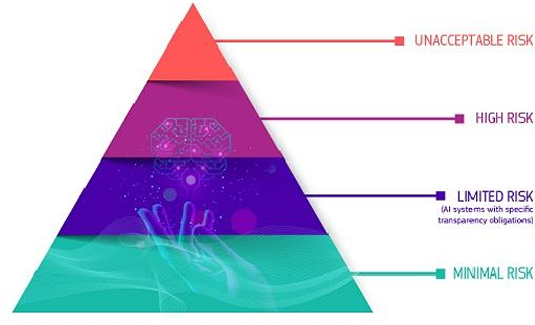
\includegraphics[width=0.6\linewidth]{images/piramide.png}
\end{figure}

\begin{itemize}
    \item \textbf{Unacceptable risk:} All AI systems considered a clear threat to the safety, livelihoods and rights of people will be banned
    \item \textbf{High risk:} \begin{itemize}
        \item critical infrastructures (e.g. transport), that could put the life and health of citizens at risk;
        \item educational or vocational training, that may determine the access to education and professional course of someone’s life (e.g. scoring of exams);
        \item safety components of products (e.g. AI application in robotassisted surgery);
        \item employment, management of workers and access to selfemployment (e.g. CV-sorting software for recruitment procedures);
        \item essential private and public services (e.g. credit scoring denying citizens opportunity to obtain a loan);
        \item law enforcement that may interfere with people’s fundamental rights (e.g. evaluation of the reliability of evidence);
        \item migration, asylum and border control management (e.g. verification of authenticity of travel documents);
    \end{itemize}
    \item \textbf{Limited risk:} refers to AI systems with specific transparency obligations
\end{itemize}

\chapter{lez 3}

\chapter{lez 4}

\chapter{lez 5}


\chapter{Intelligent transportations and Vehicle to everything protocol Examples of IoT, IoT security Artificial Intelligence of Things (AIoT), HW/SW environments for IoT/AIoT}


\chapter{Data Gathering, Data Preprocessing, Data Harmonization for intelligent system learning}

\section{Value of Data Analytic}
\begin{figure}[H]
    \centering
    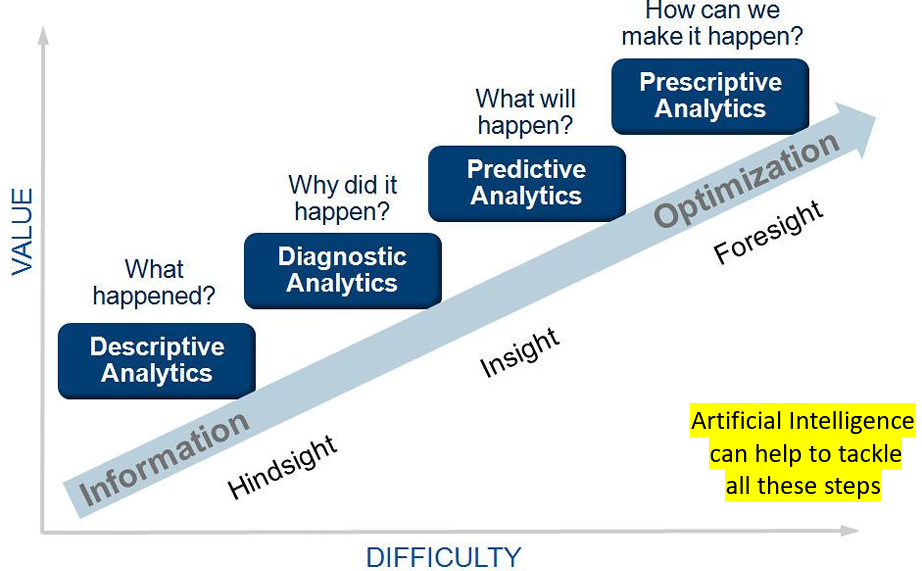
\includegraphics[width=0.8\linewidth]{images/Data.png}
\end{figure}

Four possibility increasing the value and the difficulty:
\begin{itemize}
    \item Descriptive Analytics
    \item Diagnostic Analystics
    \item Predictive Analytics
    \item Prespective Analaytics
\end{itemize}

\section{Data gathering - Step 1}
\begin{figure}[H]
    \centering
    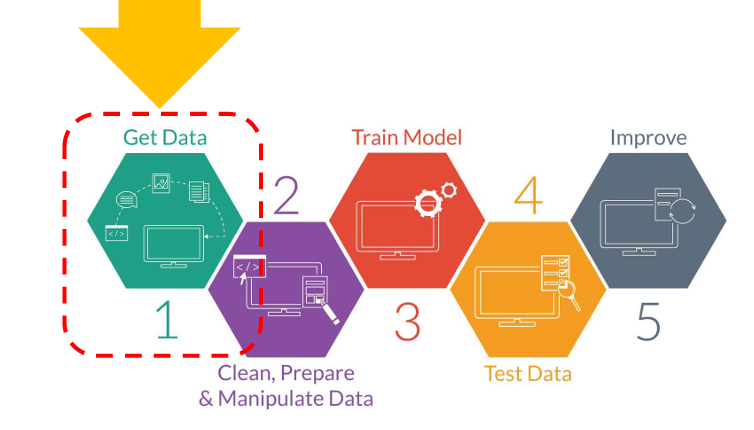
\includegraphics[width=0.8\linewidth]{images/data ghatering.png}
\end{figure}

\noindent We have so many powerful sources capable to generate data.

\noindent \textbf{Data collection is the process of gathering and measuring information on targeted variables in an established system}

\subsection{IoT started to generate data…}
\noindent The amount of data generated by connected internet of things (IoT) devices, forecast to grow to by 2025
\begin{itemize}
    \item 41.6 billion connected devices
    \item 79.4 zettabytes (ZB) of data/year.
\end{itemize} 

\noindent Data sources like phones, smart watches, ecc..

\begin{figure}[H]
    \centering
    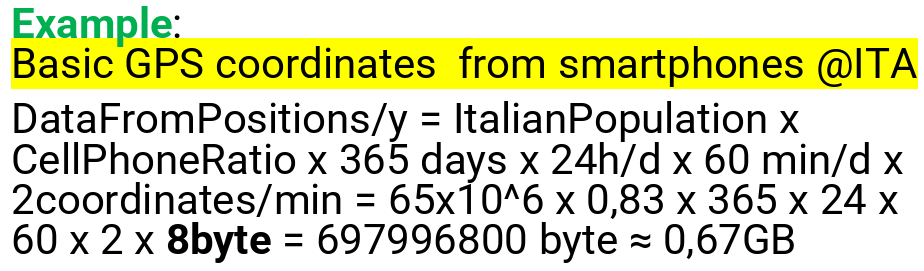
\includegraphics[width=0.8\linewidth]{images/example 1.png}
\end{figure}

\noindent There are pubblic data centers, like Amazon's, Google's and Governative's ones

\subsection{Data heterogeneity and synchronization}
\noindent  Heterogeneity in statistics means that your populations, samples or results are different. It is the opposite of homogeneity which means that the, population/data/results are the same.
Qua fa un tot di esempi  su come sia importante avere tutti i dati nello stesso formato (esempio di Marte e della NASA e della wind station)

\subsection{Data Synchronization}
\noindent The way a device adjusts its internal clock in order to align with the clocks of other devices in a network

\subsubsection{Network Time Synchronization}
Computer clocks in servers, workstations and network devices are inherently not enough accurate
Two problems:
\begin{itemize}
    \item Clocks are set by hand to within a minute or two of actual time and are rarely checked after that 
    \item Clocks are maintained by a battery-backed device that may drift as much as a second per day 
\end{itemize}
\noindent \textbf{It’s impossible to have accurate time synchronization without a proper method}

\subsubsection{Solutions}
\begin{itemize}
    \item \textbf{Network Time Protocol (NTP):} is a protocol for clock synchronization between computer systems over packetswitched, variable-latency data networks designed to mitigate local network latency 
    \item \textbf{Time Server:} Dedicated network Time Server behind your firewall (devices synchronized to within 1/2 to 2 ms)
\end{itemize}

\begin{figure}[H]
    \centering
    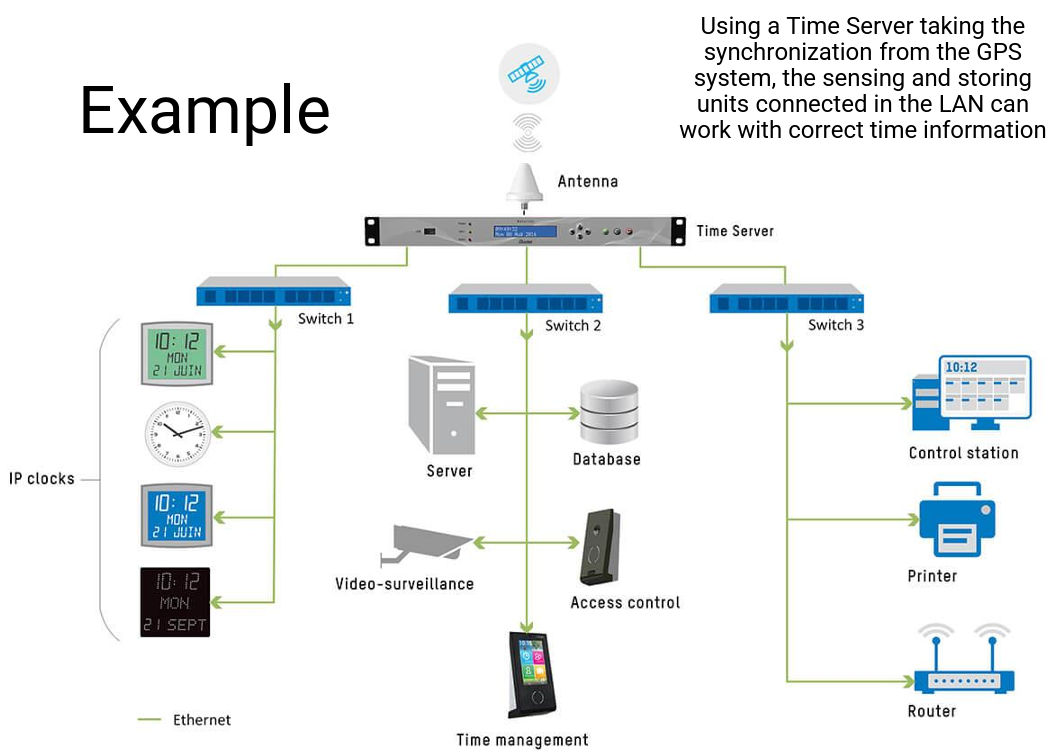
\includegraphics[width=0.8\linewidth]{images/sync.png}
\end{figure}


\section{Data Preparation - Step 2}
\begin{figure}[H]
    \centering
    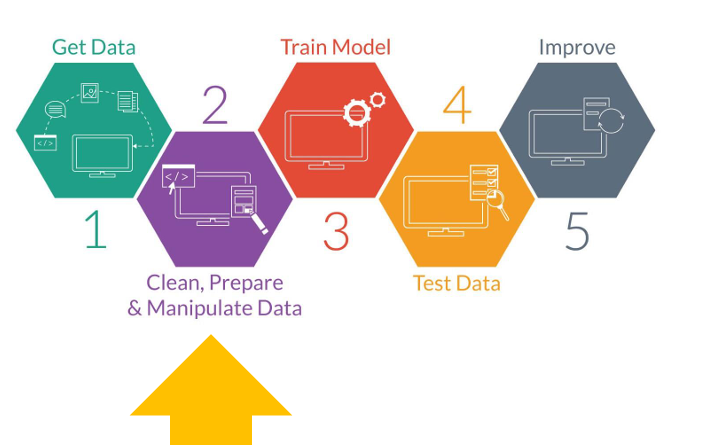
\includegraphics[width=0.8\linewidth]{images/step2.png}
\end{figure}

\noindent Data preparation includes two concepts such as Data Cleaning and Feature Engineering

\noindent The data wrangling problem is growing as different types of unstructured data or data in varying formats are pouring in from sensors, online and from traditional databases. 
All these data must be \textbf{cleaned up and organized } before data analytics/classifiers/regressors models can be applied.

\subsection{Data wrangling}
\noindent Data wrangling steps:
\begin{itemize}
    \item Iterative process
    \item Understand
    \item Explore
    \item Transform
    \item Augment
    \item Visualize
\end{itemize}

\begin{figure}[H]
    \centering
    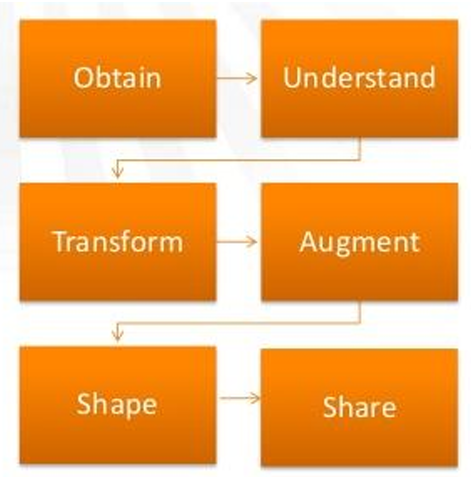
\includegraphics[width=0.6\linewidth]{images/data wrangling.png}
\end{figure}

\noindent Tasks of Data Wrangling:
\begin{itemize}
    \item \textbf{Discovering:} Firstly, data should be understood thoroughly and examine which approach will best suit. 
    \item \textbf{Structuring:} As the data is gathered from different sources, the data will be present in various shapes and sizes. Therefore, there is a need for structuring the data in proper format.
    \item \textbf{Cleaning:} Cleaning or removing of data should be performed that can degrade the performance of analysis.
    \item \textbf{Enrichment:} Extract new features or data from the given data set to optimize the performance of the applied model.
    \item \textbf{\textit{Validating:}} This approach is used for improving the quality of data and consistency rules so that transformations that are applied to the data could be verified.
\end{itemize}

\noindent \textbf{Data pre-processing:} "is a technique that is used to convert the raw data into a clean data set"
\noindent Pre-processing includes • Data cleaning • Data integration • Data transformation • Data reduction

\noindent \textbf{Why is Data Preprocessing is so important?}
\noindent Three answers:
\begin{itemize}
    \item Inaccurate data (missing data) 
    \item The presence of noisy data/erroneous data/outliers
    \item Inconsistent data 
\end{itemize}

\subsection{Missing Data}
\noindent What do we do when we have missing data? 
\begin{itemize}
    \item \textbf{Ignoring the missing record:} is the simplest and efficient method for handling the missing data (not the best method when the number of missing values are immense or  when the missing data problem and can solved (debugging/re-designredoing the experiment) and not just ignoring the problem causing the missing data.). 
    \item \textbf{Filling the missing values manually:} one of the best-chosen methods, But there is one limitation that when there are large data set, and missing values are significant then, this approach is not efficient as it becomes a timeconsuming task.
    \item \textbf{Filling using computed values:} The missing values can also be occupied by computing mean, mode or median of the observed given values (ex: you can copy from the most similar column or generate values by using any ML or Deep Learning algorithm but  it can generate bias within the data). 
\end{itemize}

\begin{figure}[H]
    \centering
    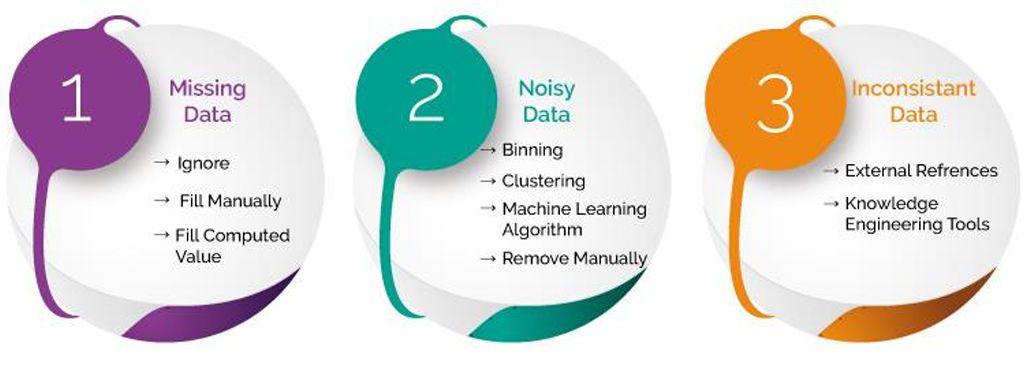
\includegraphics[width=0.8\linewidth]{images/data missing.png}
\end{figure}

\subsection{Structured and unstructured Data }
\noindent \textbf{Structured data} usually resides in relational databases, This format is eminently searchable both with human generated queries and via algorithms using type of data and field names, such as alphabetical or numeric, currency or date.

\noindent \textbf{Unstructured data} is essentially everything else. Unstructured data has internal structure but is not structured via pre-defined data models or schema (ex: sensor data, text files, emails, etc..).

\subsubsection{Neural networks and unstructured data}
\noindent It is not strictly compulsory to have structured data to use ML 

\begin{figure}[H]
    \centering
    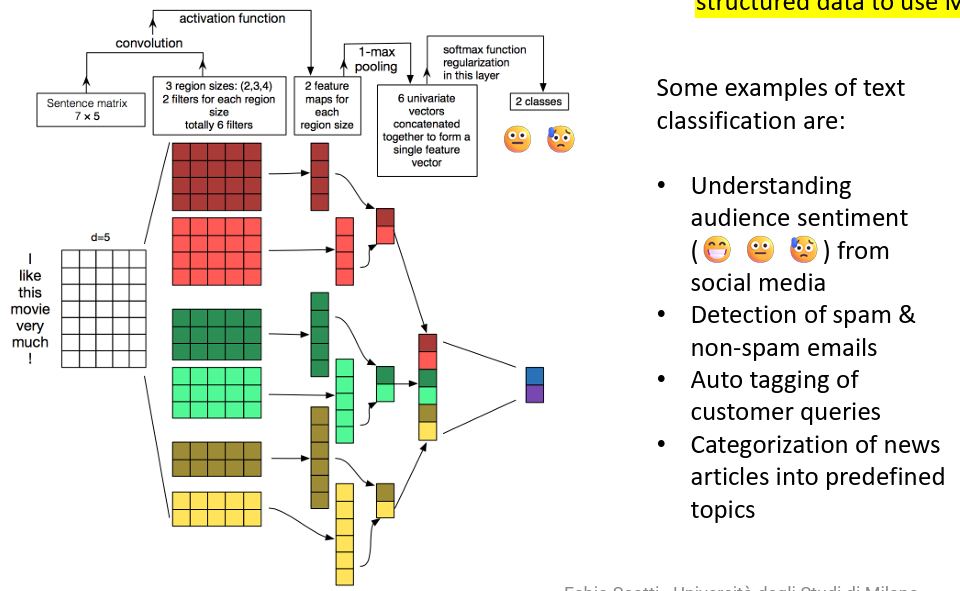
\includegraphics[width=0.8\linewidth]{images/unstructured data.png}
\end{figure}



\chapter{Managing a small dataset in Python Degrees of freedom/parameters Data Leakage}
Sta lez probabilmente fa lab però non ci dovrebbe essere lab preciso all'esame 
Lo fa sul link delle slide

\end{document}